\chapter{Implementation of Improved HeidelTime Multilingual Model} \label{the-chapter-4}
In this chapter, we present the implementation of our improved multilingual model for HeidelTime. The starting point of our work, is the model presented by  Str\"{o}tgen and Gertz in \cite{DBLP:conf/emnlp/StrotgenG15}, and also discussed in Section \ref{multilingual-ht-model} of this thesis. We extend the model to address its issues we discussed in Section \ref{improved-multilingual-ht-model}. In this chapter, we discuss the implementation details of our improved model. 

In Section \ref{sec4a}, we discuss the external data sources we use. In Section \ref{sec4b}, we describe how inflections are incorporated. In Section \ref{sec4c}, we discuss how rules for unsegmented languages are adjusted. In Section \ref{sec4d}, we explain the learning of language specific rules. 

%	\textcolor{violet}{some intro ...}

\section{Data Sources} \label{sec4a}
We use external sources such as online dictionaries and word embeddings to get inflections for morphologically-rich languages. Moreover, to learn language specific frequently occurring patterns as rules, we use Wikipedia. 


\subsection{Wiktionary}
Wiktionary, made available by the Wikimedia Foundation, is a \textit{web-based project to create a free content dictionary of all words in all languages}\footnote{\url{https://en.wikipedia.org/wiki/Wiktionary}}. Like other sites of Wikipedia, it is collaboratively edited via wiki by volunteers, that are not necessarily language experts. The content of a usual Wiktionary article may give information about a word's part-of-speech, etymology, definitions, example usage sentences, pronunciations, translations, synonyms/antonyms, among others \cite{navarro2009wiktionary}. For certain words of morphologically-rich languages, inflections may also be provided.
	
The translation section for a word on Wiktionary article can contain multiple translation tables, if the word has more than one meanings in English. For instance, the month name ``May" has more than one meaning in English, i.e., the fifth month of the Gregorian calendar, the name of a hawthorn flower or a given name; so the English wiktionary page for May has three translation tables\footnote{\url{https://en.wiktionary.org/wiki/May\#Translations}}, one for each of the mentioned meaning. These are the translation tables, that are used by the present HeidelTime multilingual model \cite{DBLP:conf/emnlp/StrotgenG15} to extract translations in various languages (the third step in Figure \ref{figure:3d}).
	
As mentioned earlier, Wiktionary may also provide inflection tables, for words that have inflections. Continuing from the example of the English wiktionary page for the word ``May", in the translation table for the sense, i.e., fifth month, translations in various languages are given. For instance, next to Turkish, the translation is given as ``mayıs", that points to its own page\footnote{\url{https://en.wiktionary.org/wiki/may\%C4\%B1s\#Turkish}}, that describes the word ``mayıs", and also provides an inflection table for it. As the present HeidelTime multilingual model already gets the translation ``mayıs" from the page for May, the next step should be to extend it further so as to also get the inflections for the word ``mayıs'' from its page. 

On analysing Wiktionary, we found that it provided inflections tables for the words in languages such as Finnish, Turkish, Polish, etc.  The words in these languages we looked for were the translations in respective languages for the words as given in the simplified English normalization resources (Subsection \ref{res-ir} \ref{res-ir-i}). For instance, the month names in Finnish, Turkish and Polish all had inflection tables available on Wiktionary. 
	
\subsection{FastText}
FastText\footnote{\url{https://fasttext.cc/}}, by Facebook Research, is a highly multilingual library for efficient learning of word representations and text classification. FastText is a library that provides word embeddings, also known as word vectors or distributed representation, for words. Word embedding libraries embed words in a vector space model, thereby representing each word by a vector, such that semantically similar words have vectors that are closer to each other. 

FastText learns representations for character n-grams, and represent words as as the sum of the learnt character n-gram vectors \cite{DBLP:journals/tacl/BojanowskiGJM17}. FastText takes into account the morphology of words by having many vectors for different parts of a word (n-grams). In addition to utilizing character level information to improve word vectors, FastText also has made available pre-trained word vectors for 294 languages\footnote{\url{https://fasttext.cc/docs/en/pretrained-vectors.html}}. 

FastText has been shown to perform on par with recent deep learning methods in the tasks of text classification and sentiment analysis, while being much faster \cite{DBLP:journals/corr/JoulinGBM16}. Similarly, it was also shown to perform very well for the tasks of word similarity and word analogies \cite{DBLP:journals/tacl/BojanowskiGJM17}. 

FastText also provides an interface to find the nearest neighbors of a word. Given a word as input, it returns a list of similar words ranked by their cosine similarity scores. This can be used to get interchangeable words for a word, or to simply validate the quality of learnt word vectors by looking at the nearest neighbors for some words. We looked at the nearest neighbor functionality for languages such as Finnish, Estonian and Turkish, and found out that it consistently returning the inflections of words in the list of top ten nearest neighbor words, though related words that are not inflections were also returned.

\subsection{Wikipedia}
Wikipedia, made availabe by the Wikimedia Foundation, is a \textit{free online encyclopedia with the mission of allowing anyone to edit articles}\footnote{\url{https://en.wikipedia.org/wiki/Wikipedia}}. It is available in 299 languages, and is ranked fifth most popular website\footnote{\url{http://www.alexa.com/siteinfo/wikipedia.org}}. Of the 299 languages Wikipedia is available in, 13 of these have over one million articles each\footnote{\url{https://en.wikipedia.org/wiki/Wikipedia\#Language\_editions}}. Full details about the number of articles available in each language can be seen at the link\footnote{\url{https://meta.wikimedia.org/wiki/List\_of\_Wikipedias}}.

Wikipedia has made available the dumps\footnote{\url{https://dumps.wikimedia.org/}} in various formats such as XML, SQL, etc. These can be downloaded for all the languages Wikipedia is available in. We aim to make use of these dumps for the tasks of learning frequently occurring temporal expressions for different languages and for the analysis of languages that lack temporally annotated coropora. 
\section{Getting Inflections} \label{sec4b}
As mentioned earlier, in Section \ref{morphologically-rich-languages-background} (page \pageref{morphologically-rich-languages-background}), morphologically-rich languages are such that have rich morphology of words in them or inflection of words. As of HeidelTime version 2.2.1, the pattern resources of current HeidelTime do not have the inflections of words in them for such languages. This renders the useful rules, in language independent rules for such languages, useless as they are not able to extract patterns due to missing inflections in respective pattern resources.  

For instance, a simple date rule, in automatically developed resources for extracting dates like ``16 August 2003" with punctuations and few tokens allowed in between is given in the following listing. \\

% zebra color effect following commented lines, but the mess up referencing labels of these lstings	
%\begin{lstlisting}[
%caption={A language independent rule to extract dates - showing only extraction part of the rule},
%label={listing:4a}
%identifierstyle=\oddtest,
%commentstyle=\oddtest,
%stringstyle=\oddtest,
%keywordstyle=\oddtest,
%linebackgroundcolor={\ifodd\value{lstnumber}\color{cream}\fi}
%]
%// r1a: 30 August 2000 (with "." and "," etc allowed between)
%%reDayNumber\.?( [\S][\S]?)? %reMonthName,?( [\S][\S]?)? %reYear4Digit
%\end{lstlisting}

\begin{minipage}{\linewidth}
\begin{lstlisting}[
caption={A language independent rule to extract dates - showing only extraction part of the rule.},label={listing:4a}]
// r1a: 30 August 2000 (with "." and "," etc allowed between)
%reDayNumber\.?( [\S][\S]?)? %reMonthName,?( [\S][\S]?)? %reYear4Digit
\end{lstlisting}
\end{minipage}


Now let us consider the following Finnish text\footnote{The Finnish text excerpt is taken from Wikipedia, see \url{https://fi.wikipedia.org/wiki/?curid=30}}:

%\begin{figure}[H]
%	\centering
	\begin{mdframed}[style=MyFrame]
		\raggedright{
			Antti Johannes Satuli (\ul{8. lokakuuta 1946} Helsinki – \ul{17. huhtikuuta 2003} Inari) oli oikeustieteen kandidaatti, joka loi uransa Suomen ulkoasiainministeriön palveluksessa. Hän oli Suomen ensimmäinen suurlähettiläs ja pysyvä edustaja Euroopan unionissa siihen liittymisen jälkeen. Vuonna 2002 hänet nimitettiin ulkoministeriön valtiosihteeriksi.
		}
	\end{mdframed}
%	\caption{a sample Finnish text excerpt}
%	\label{figure:4-finnish-text-excerpt}
%\end{figure}

We can see that above Finnish excerpt has two dates in it that are underlined. The rule given in Listing \ref{listing:4a} is perfectly capable of extracting the dates underlined in above given Finnish text. However, these dates are not extracted by the HeidelTime as of version 2.2.1, as the month names in those dates, i.e., ``lokakuuta" and ``huhtikuuta" are inflections of the nominative forms, i.e., ``lokakuu" and ``huhtikuu" respectively. Since, only the nominative forms of months are present in Finnish reMonthName pattern file for Finnish, as of HeidelTime 2.2.1, these dates are not extracted (see\footnote{The inflection and cases information about month names in Finnish language being discussed here is taken from wiktionary: \url{https://en.wiktionary.org/wiki/huhtikuu\#Finnish} and \url{https://en.wiktionary.org/wiki/lokakuu\#Finnish}; we are not native speakers of the language}). 

If reMonthName for Finnish is created such that it has the inflections in it the same rule given in Listing \ref{listing:4a} will successfully extract the underlined temporal expressions in sample Finnish text given above. We aim to create pattern files such that they contain such inflections for morphologically rich languages. 

We make use of the external sources of Wiktionary and FastText to get inflections, and put them in pattern resources of automatically developed resources for HeidelTime. 

\subsection{Getting Inflections Using Wiktionary} \label{sec4b1}
The first approach we take to get inflections is to use Wiktionary as a data source. This approach can be considered as a direct extension of the current Multilingual HeidelTime model, discussed in Section \ref{multilingual-ht-model} (page~\pageref{multilingual-ht-model}), to create automatically developed resources. We extend the multilingual model to get inflections for the words we are translating, if they exist. 

For the sake of completeness, below we restate all the steps with our extension step (\ref{extension-step-3a}):

\begin{enumerate}[1.]
	\item We create pattern and normalization resources, for each language, using the language dependent resources. These pattern and normalization resources are empty at the end of this step.
	\item We then get all the patterns (English words to translate) from the language dependent resources. 
	\item We then crawl each respective Wiktionary page of the patterns (English words to translate) and get the translation for the patterns from the translation tables present on Wiktionary. For instance, for month name January, we get the translation tammikuu for Finnish language in this step. Similarly, we get translations for all the pattern words in all languages.  
		\begin{enumerate}[a.]
		\item \label{extension-step-3a} This step is the extension we add to current multilingual model of HeidelTime. Here we crawl the page of respective translations of the patterns, and get all inflections from the inflection table if they exist. For instance, for Finnish language, we go to the Wiktionary page for ``tammikuu'', and get all its inflections such as tammikuut, tammikuun, etc. from its inflection table. Similarly, we get inflections for other words and for other languages. 
		\end{enumerate}
	\item We then fill the empty pattern and normalization files, created in first step, with the found translation words and their inflections. 
	\item Finally, we add the language independent resources and language independent rules to the created resources for each language in previous step to get the final automatically developed resources for all languages. 
\end{enumerate} 

The following figure gives an overview of all these steps to create automatically developed resources. It is identical to the Figure \ref{figure:3d} (page~\pageref{figure:3d}), except for the additional step that is shown as highlighted. 

\begin{figure}[H] 
	\centering
	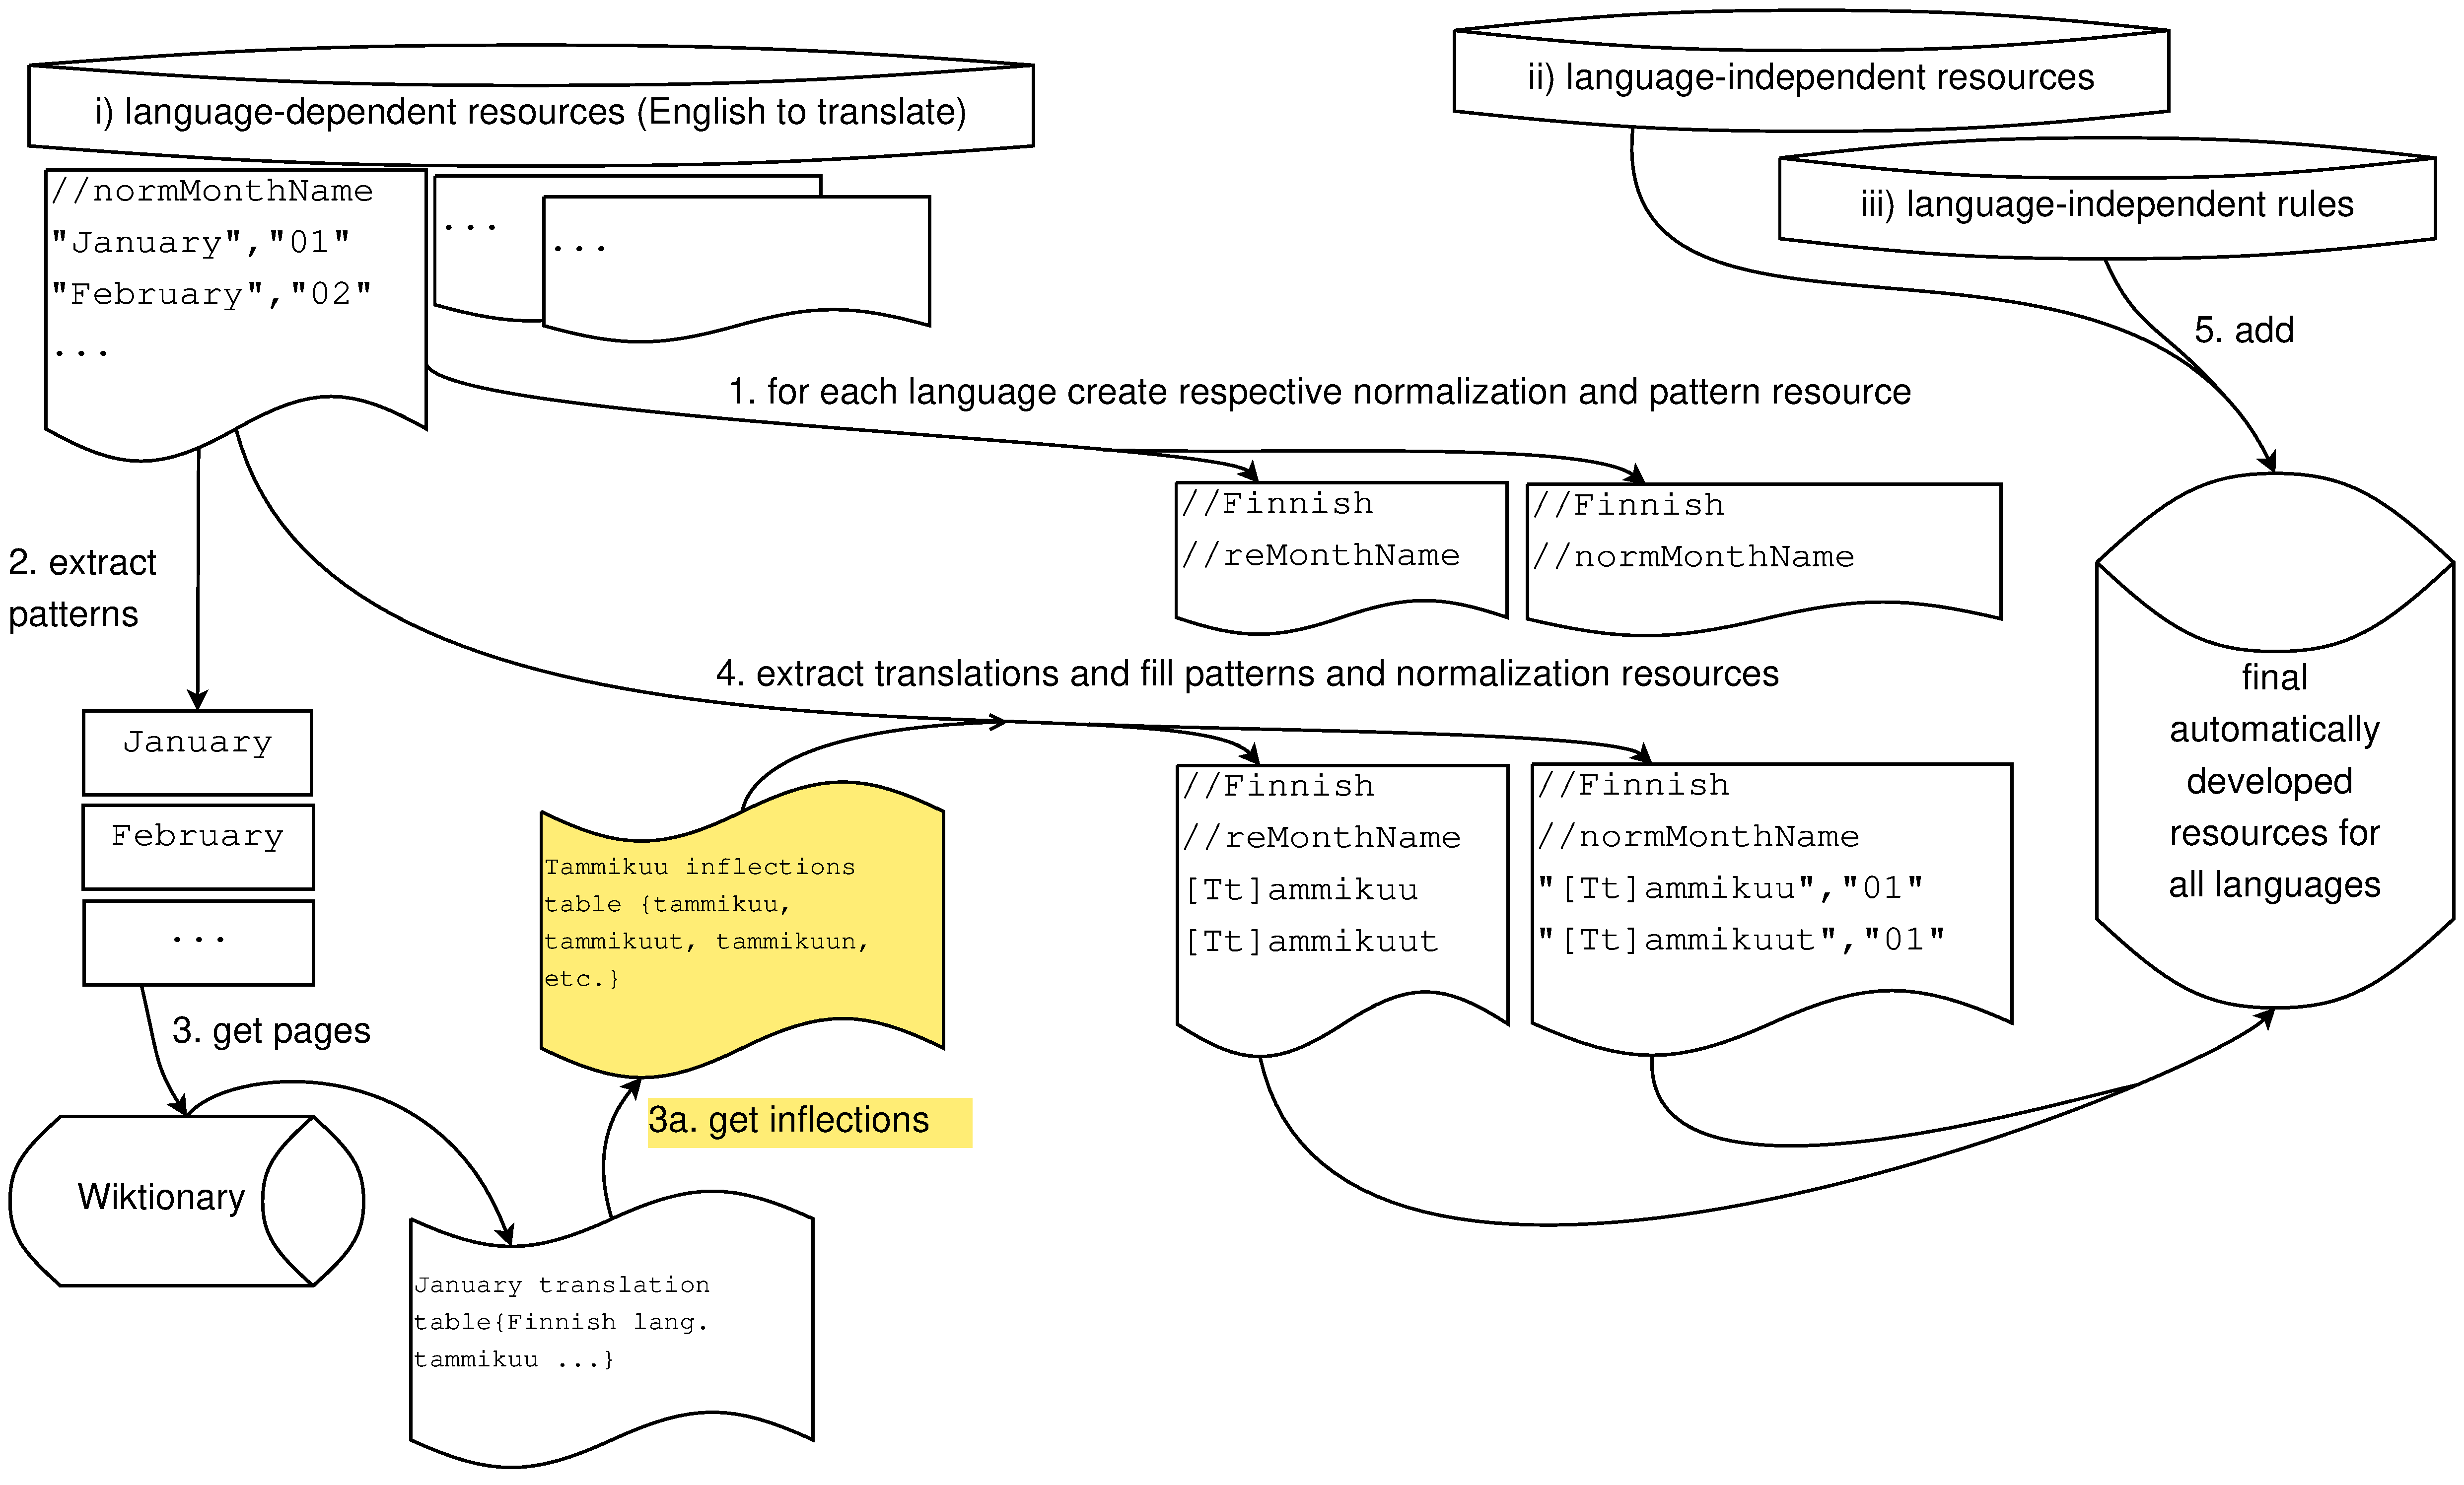
\includegraphics[width=14cm]{Graphics/ht-multilingual-new-1}
	\caption{Overview of Improved Mutlilingual HeidelTime Model - Getting Inflections - using Wiktionary.}
	\label{figure:4a}
\end{figure}

\textbf{Resulting Resources}\\
Once we run the improved multilingual model discussed above, we get the automatically developed resources for all languages contain inflections in their pattern and normalization files. We observed the resulting pattern files for morphologically rich languages and found that the inflections were successfully extracted from Wiktionary. For instance, the Listing \ref{listing:4-fi-2x-wiktionary} below shows part of pattern file reMonthName for Finnish language using our new improved multilingual model:\\


%\begin{figure}[H]
%	\centering
%	\includegraphics[width=8cm]{fi-reMonthName-ht-2x-wiktionary}
%	\caption{reMonthName for Finnish language - using Improved Multilingual HeidelTime Model - using Wiktionary}
%	\label{figure:4b}
%\end{figure}

\begin{minipage}{\linewidth}
\begin{lstlisting}[caption={reMonthName for Finnish language - using Improved Multilingual HeidelTime Model - using Wiktionary.},label={listing:4-fi-2x-wiktionary}]
// english: January, 01
[Tt]ammikuu
[Tt]ammikuusta
[Tt]ammikuiden
[Tt]ammikuuksi
[Tt]ammikuissa
[Tt]ammikuitten
[Tt]ammikuuhun
// ...
\end{lstlisting}
\end{minipage}

We can see that our improved model extracted all the inflections for month name ``Tammikuu", as compared to the only base word ``Tammikuu" being extracted by the multilingual model, as of HeidelTime version 2.2.1 (c.f. Listing \ref{listing:3-fi-reMonthName-ht-221}, page \pageref{listing:3-fi-reMonthName-ht-221}). 
\subsection{Getting Inflections Using FastText} \label{sec4b2}
The second approach we take to get inflections is to use FastText's nearest neighbor functionality. The overall model is again similar to the original model, except now instead of Wiktionary we make use of Yandex.Translate\footnote{\url{https://translate.yandex.com/}} service and FastText library. We use Yandex online translator instead of other translators such as Google or Microsoft because it is available freely; moreover, we also get to create resources developed using a resource other than Wiktionary. In addition, we use FastText because it is an open-source and lightweight library that provides multilingual word vectors for over 150 languages; and provides functionality that returns nearest neighbors of an input word, which we aim to use to get inflections of words in morphologically rich languages.

Following, we only state the steps that are performed differently than when getting inflections using Wiktionary model.

\begin{enumerate}[1.]
	\setcounter{enumi}{2}
	\item For each of the patterns (English words to translate), get their translation from Yandex Translate. For instance, for month name January, we get the translation Tammikuu for Finnish in this step. Similarly, we get translations for all the pattern words for all languages. 
	\begin{enumerate}[a.]
		\item Here we take the translation we got from previous step and get nearest neighbors of the translation using FastText. For instance, for the translated word Tammikuu in Finnish, we get some relevant inflections for it such as Tammikuulla, and we also get some relevant words but not inflections such as Helmikuu (February in Finnish language).  
		\item As some relevant words might be returned by FastText that are not inflections, so we translate the returned words again using Yandex Translate, and verify if they indeed translate back to the original pattern. For instance, the returned relevant inflection word Tammikuulla by FastText will translate back to January; however, the returned relevant word but not inflection, i.e., Helmikuu, will not translate back to January. 
	\end{enumerate}
\end{enumerate}

The rest of steps are similar to the model to get inflections using Wiktionary (Figure \ref{figure:4a}). The following figure gives an overview of all these steps to create automatically developed resources using FastText. It is identical to the Figure \ref{figure:4a} (page~\pageref{figure:4a}), except for the highlighted steps. 

\begin{figure}[H] 
	\centering
	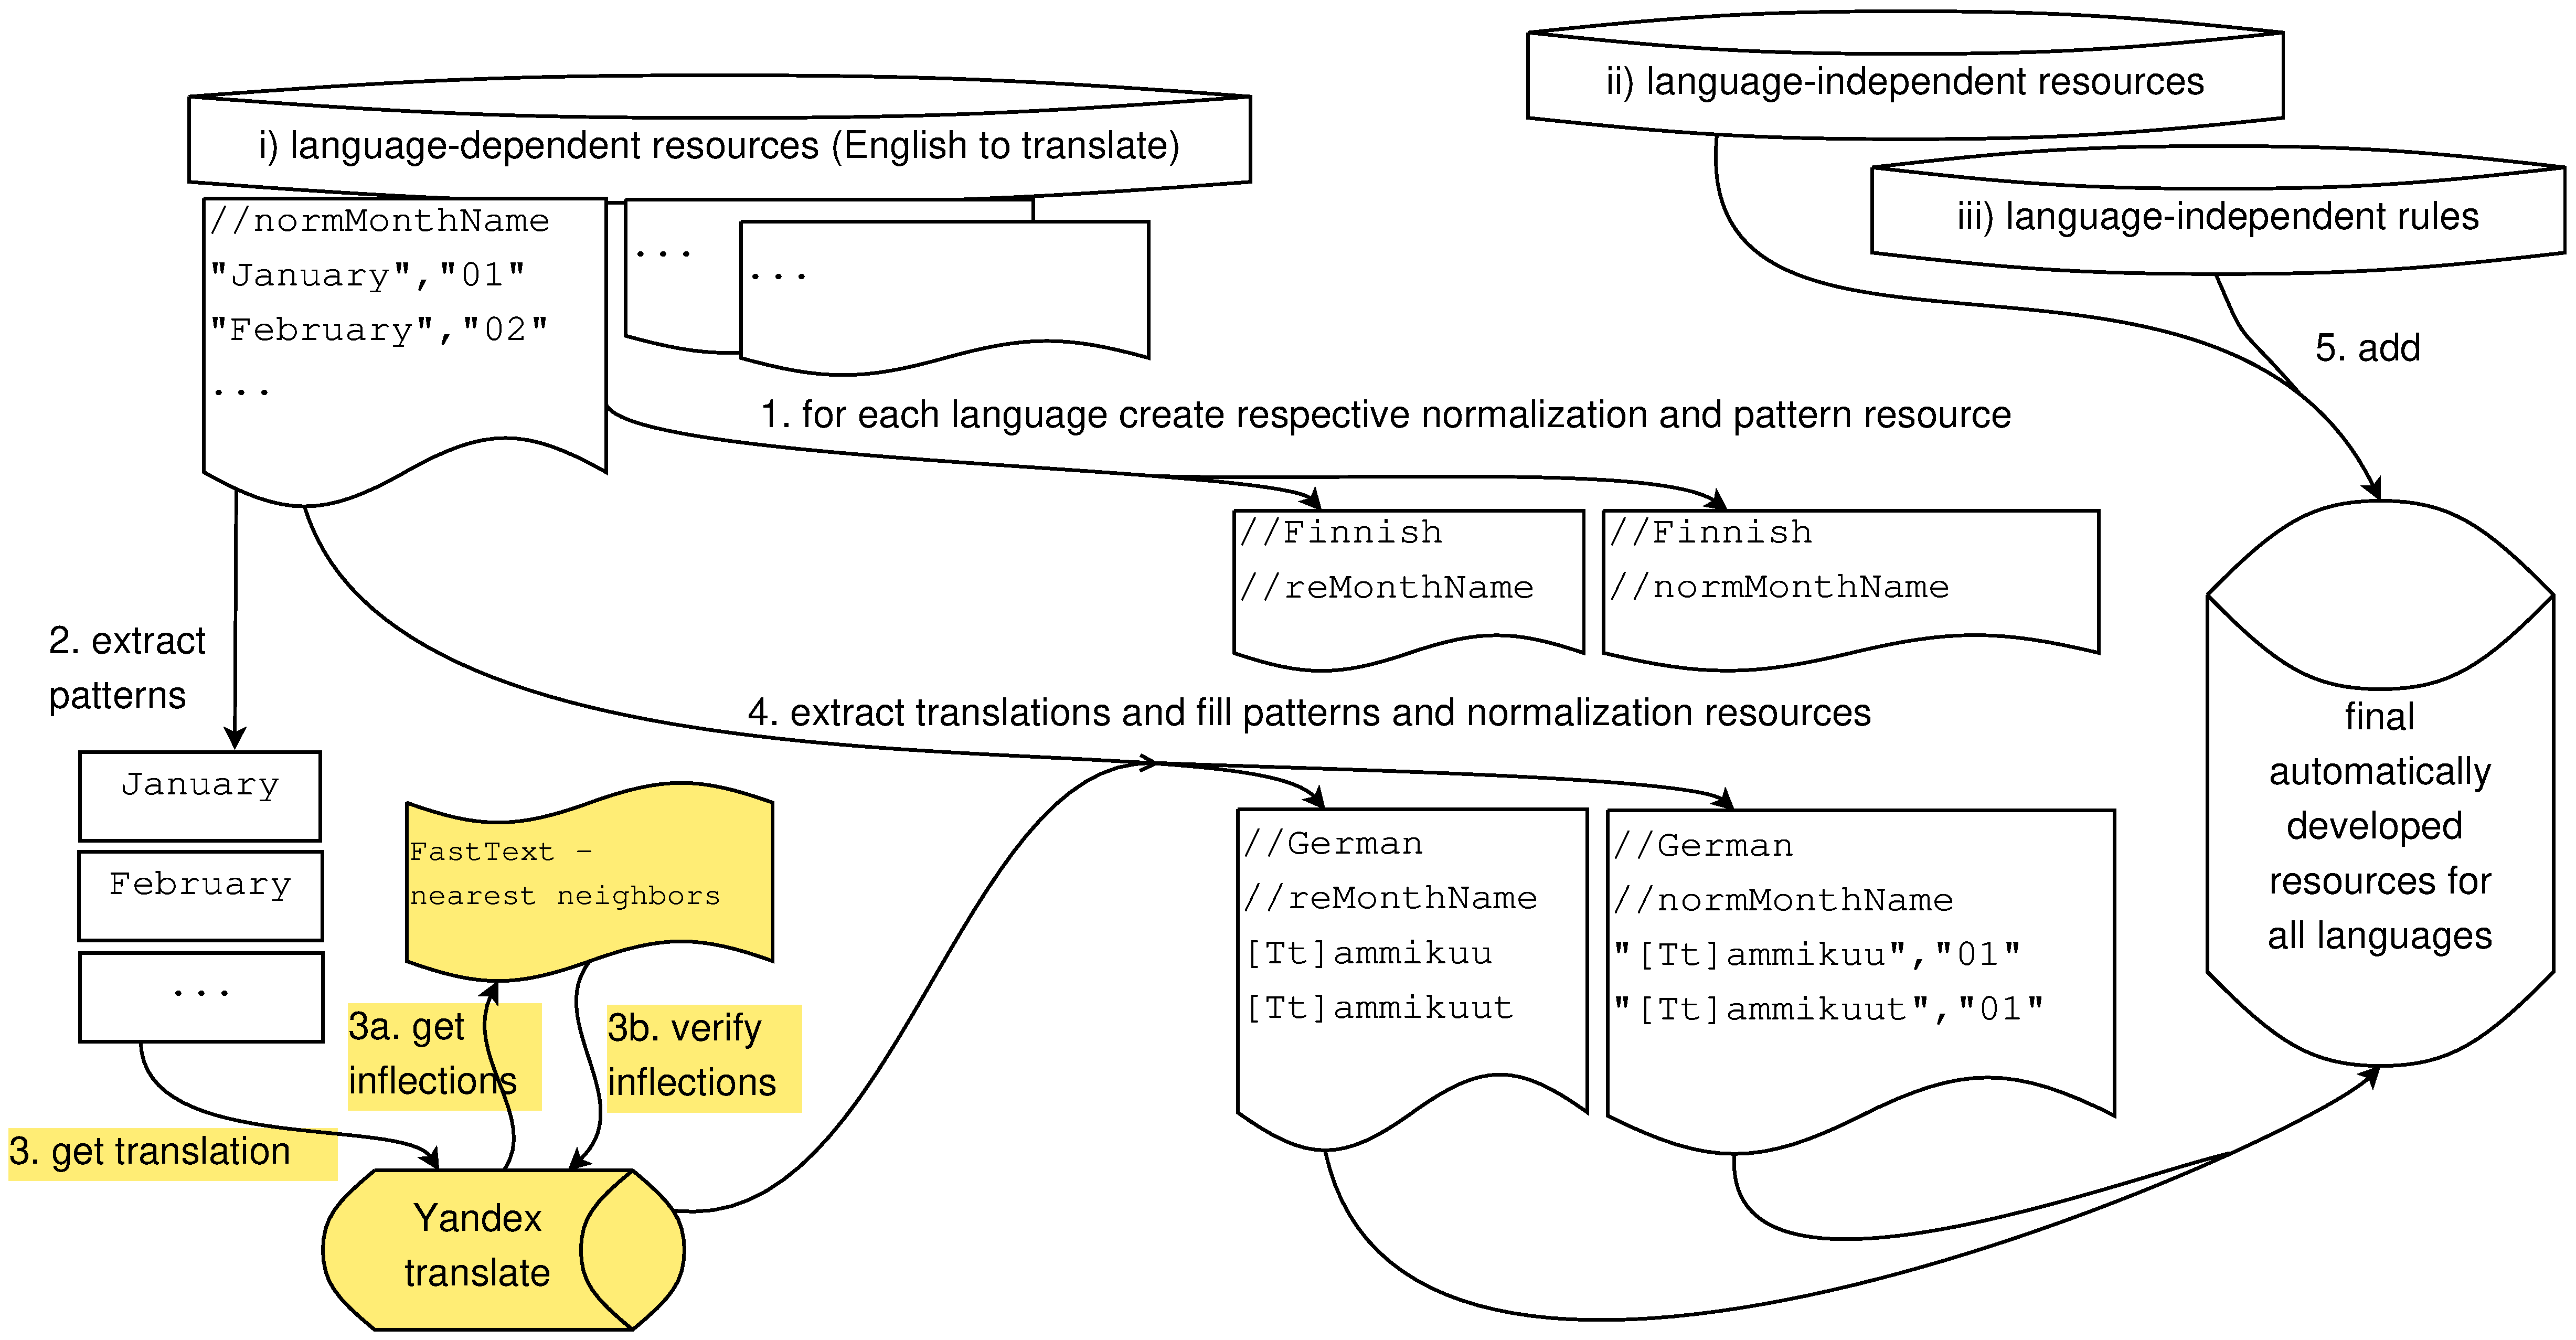
\includegraphics[width=14cm]{Graphics/ht-multilingual-new-2}
	\caption{Overview of Improved Mutlilingual HeidelTime Model - Getting Inflections - using FastText.}
	\label{figure:4c}
\end{figure}

\textbf{Resulting Resources}\\
Once we run the improved multilingual model discussed above, using word vectors of a certain language, we get the automatically developed resoruces for that language. The created pattern and normalization resources have inflections in them for morphologically rich languages. We compared the resulting resources for some of the morphologically rich languages and found that, though inflections were being extracted and written in resources, they were less in number than those obtained by the earlier model that used Wiktionary as a data source to get inflections. For instance, the following Listing \ref{listing:4-fi-2x-ft} shows part of pattern file reMonthName for Finnish language that is created using our improved multilingual model that uses FastText as data source:\\

\begin{minipage}{\linewidth}
\begin{lstlisting}[caption={reMonthName for Finnish language - using Improved Multilingual HeidelTime Model - using FastText.},label={listing:4-fi-2x-ft}]
// english: "January","01"
[Tt]ammikuu
[Tt]ammikuuta
[Tt]ammikuut
// english: "February","02"
[Hh]elmikuuta
[Hh]elmikuu
[Hh]elmiku
// ...
\end{lstlisting}
\end{minipage}

We can see that even though inflections are extracted, but they are less than the number of inflections in Finnish rePatternFile file created using earlier model that used Wiktionary (c.f. Listing \ref{listing:4-fi-2x-wiktionary}). It might be the case that FastText method gives us better rePattern files for some languages as compared to the Wiktionary method; this will be discussed in the evaluations we run in the Chapter \ref{the-chapter-5}.

\section{Accommodating Unsegmented Languages} \label{sec4c}
As of HeidelTime version 2.2.1, the automatically developed resources of all languages use the same language independent rules. These rules are simplified rules and use space as a separator between different temporal expressions in a rule. 

For instance, extraction part of a simple date rule in the simplified rules is:\\


%\begin{lstlisting}[
%caption={A simple language independent rule to extract dates - showing only extraction part of the rule},label={listing:4b}
%identifierstyle=\oddtest,
%commentstyle=\oddtest,
%stringstyle=\oddtest,
%keywordstyle=\oddtest,
%linebackgroundcolor={\ifodd\value{lstnumber}\color{cream}\fi}
%]
%%reMonthName %reDayNumber,? %reYear4Digit
%\end{lstlisting}

\begin{minipage}{\linewidth}
\lstset{caption={A simple language independent rule to extract dates - showing only extraction part of the rule.},label={listing:4b}}
\begin{lstlisting}
// rule to extract dates like January 20, 2002
%reMonthName %reDayNumber,? %reYear4Digit
\end{lstlisting}
\end{minipage}

%\begin{mdframed}[style=MyFrame]
%	\begin{verbatim}
%	%reMonthName %reDayNumber,? %reYear4Digit
%	\end{verbatim}
%\end{mdframed}

The rule in Listing \ref{listing:4b} extracts temporal expressions that appear in following order, i.e., reMonthName followed by space followed by reDayNumber followed by an optional comma followed by space and finally reYear4Digit. Thus, we can see this rule assumes space as separator between the parts of a date. This extraction pattern ignores the unsegmented languages and would not extract temporal expressions in such languages. We refer to similar date rule for Chinese language, as given in manually created Chinese resources of HeidelTime \cite{DBLP:conf/eacl/LiSZG14}. The similar rule in Chinese given in manual HeidelTime resource is:\\

\begin{minipage}{\linewidth}
\lstset{caption={A manually developed Chinese rule to extract dates - showing only extraction part of the rule.},label={listing:4c}}
\begin{lstlisting}
// EXAMPLE date_year_c5: 一九八七十二月二十八日
(%reYear4Digit|%reYear2Digit)年(%reMonthWord)(%reDayWord日)
\end{lstlisting}
\end{minipage}

%\begin{mdframed}[style=MyFrame]
%	\begin{verbatim}
%	%reYear4Digit年%reMonthWord%reDayWord日
%	\end{verbatim}
%\end{mdframed}

%\begin{figure}[H]
%	\centering
%	\begin{mdframed}[style=MyFrame]
%		\begin{verbatim}
%		%reYear4Digit年%reMonthWord%reDayWord日
%		\end{verbatim}
%	\end{mdframed}
%	\caption{a Chinese date rule}
%	\label{figure:4-chinese-date-rule}
%\end{figure}


In Listing \ref{listing:4c}, we see that the actual manual Chinese rule has separator words between the rePatterns (\%reYear4Digit, \%reMonthWord and \%reDayWord). The separator words used are 年 and 日, where 年 translates to `year' and 日 translates to `day'. 

Our first approach to cater the unsegmented languages is to simply remove the spaces in the simplified language independent rules for such languages, but as we can see from the above example, the space might be replaced by actual words like 年 and 日, at least in one of the complete date rule. In the next section, we present our approach to learn frequently occurring temporal patterns as rules for all languages, that might enable us to learn better rules for unsegmented languages too (For instance, a rule similar to the one in Listing \ref{listing:4c} for Chinese language). 

\section{Learning Language-specific Rules} \label{sec4d}
In this section, we discuss how the new rules are learned for different languages from frequently occurring temporal expressions in them. The learnt language specific rules are then appended to the language independent rules. The aim is to enrich the simplified language independent rules for automatically developed resources of all languages with language-specific rules of respective languages. Another way to put it is that the aim is to learn some language dependent rules by analysing Wikipedia dumps of respective languages, and append those to the simplified language independent rules. Thus, making the simplified rules language dependent and improving extraction quality. That is, the new rules will be language dependent, but as the previous extension to new languages, automatically created.

One issue with the language independent rules, for automatically developed HeildelTime resources, is that they do not have a rule for dates that have year granularity. Since using just four digit numbers might be too ambiguous and thus result in many false positives, and, without language specific information, no extended rules can be added. For instance, the temporal expressions that represent four-digit years, without month information, such as ``2004" are not extracted for any language. This is an understandable decision, because it is not necessary that every four digits refer to a year. For instance, in ``there were around 2000 spectators", 2000 does not represents the year 2000. However, if the four-digit years occur near the keyword ``year", then the four-digit number certainly refers to respective year, and is a temporal expression that should be extracted. One of our goal, in learning language specific rules, is to learn such only year rules. 

It is likely that only year rule will be a permutation of the patterns ``reYearToken" and ``reYear4Digit" and possibly some other word or punctuation. For instance, in German language the extraction part of only year rule should be:\\
\framebox{\%reYearToken \%reYear4Digit}\\
This can extract German temporal expressions such as ``Jahr 2009", assuming reYearToken pattern has the translation ``Jahr" available in it. 

It is equally likely that the four-digit year appears with some word other than the year token; for instance, in English consider the sentence ``He was born in 1934". Here the four-digit year appears with the English word ``in". As of HeidelTime version 2.2.1, there is no pattern file in English-to-translate initial resources that has word ``in" in it. Moreover, even if such file is present, there is a chance that no correct translation for any language is found while creating pattern resources for that language using Wiktionary or FastText. For instance, the Finnish word ``vuonna" translates to ``in the year"\footnote{using Wiktionary, i.e., \url{https://en.wiktionary.org/wiki/vuonna}} in English language. And the word ``vuonna" is not found by our system on wiktionary while crawling it, i.e., no pattern resource file of Finnish has the word ``vuonna" in it; so for such cases, only year rules can be made that have the word of a language itself in the rule, as compared to \%rePattern names. For instance, in Finnish language only year rule's extraction part can be:\\
\framebox{[Vv]uonna \%reYear4Digit }\\
This can extract Finnish temporal expressions such as ``vuonna 1984".

Another rule that can be learned is the complete date rule for unsegmented languages. As discussed in Section \ref{sec4c}, the simplified language independent rules do not work on unsegmented languages, because these rules assume space a delimiter between date parts or some other punctuations or small words. For instance, we aim to learn rule such as the one shown in Listing \ref{listing:4c} for Chinese language, that uses the Chinese words, i.e., 年 and 日, as separators between date parts. 

Now, we discuss our approach of analysing Wikipedia dumps for different languages to learn language dependent rules based on frequently occurring temporal expressions in respective languages. 

\subsection{Learning Language-specific Rules using Wikipedia}
The approach we take to learn language specific rules for different languages makes use of Wikipedia as a data source. As mentioned earlier, Wikipedia articles have ample temporal information in them and are readily available to download as dump files for different languages. We used the Wikipedia dumps having version 20171020 (dated 2017-10-20), for 177 languages that had this version available to download, to learn language-specific rules for these languages.

Following, we discuss our pipeline to learn rules from frequently occurring temporal expressions. 

\begin{enumerate}[1.]
	\item We get the Wikipedia dump of a language from Wikipedia dumps website\footnote{\url{http://dumps.wikimedia.your.org}}, that are in .xml.bz2 format\footnote{for instance, the Finnish wiki dump we used is available at  \url{http://dumps.wikimedia.your.org/fiwiki/20171020/fiwiki-20171020-pages-articles-multistream.xml.bz2}}, and run a script\footnote{script by Giuseppe Attardi, available at \url{https://github.com/attardi/wikiextractor}} that extracts the texts from the dumps and add them to a MongoDB collection of respective language. 
	
	\item We then set up HeidelTime UIMA pipeline, that we use to tag the Wikipedia articles of respective language's MongoDB collection, using base rules (language independent rules that have individual \%rePatterns as extraction part, see Listing \ref{listing:4d} below). This step tags all the individual temporal patterns found and puts the result in a new collection in MongoDB.
	
	\item  We then analyse the collection created in previous step. It has all the individual temporal expressions tagged separately using base rules. For instance, if two or more temporal expressions appear in close proximity of one another, we note the words or punctuations that appear between these temporal expressions. A dictionary like structure is made that has a tuple as key, that has the two contributing temporal expressions, and has dictionary as value that stores the words and their counts they appear between the two temporal expressions (see Listing \ref{listing:4e}). Similar dictionary structures to maintain the words that appear before and after an extracted  individual temporal pattern are also made. 
	
	Only the most frequently occurring word or punctuation between two indivdual temporal expressions is used as token between the contributing temporal patterns for the new rule; this makes sure that the learned rules are of quality. It should be noted that only the first 100,000 temporal expressions of each language collection, created in step 2, are analysed to learn rules. If the number of individual temporal expressions is less than 100,000 then all of the temporal expressions are analysed to learn rules. This phase learns the extraction parts of the rules and stores them in an output JSON file.
	
	\item  We then parse the JSON file from previous phase and make complete rule, in HeidelTimes rule syntax, from each rules extraction part learned in previous step. Once a complete rule, i.e., that has rule name and rule normalization part in addition to the extraction part is made, we append this rule into the rules resources for the respective language, hence making language independent rules richer with added language dependent rules. 
\end{enumerate}

The following listing depicts some of the base rules, they are basically all the rePatterns as individual rules. So each temporal pattern is extracted separately.\\

\begin{minipage}{\linewidth}
\lstset{caption={Some sample base rules.},label={listing:4d}}
\begin{lstlisting}
// br1 to extract individual patterns reDayToken, e.g., day 
RULENAME="br1",EXTRACTION="%reDayToken",NORM_VALUE="temp"
// br2 to extract individual patterns reMonthName, e.g., January, 
RULENAME="br2",EXTRACTION="%reMonthName",NORM_VALUE="temp"
// br3 to extract individual patterns reMonthToken, e.g., month 
RULENAME="br3",EXTRACTION="%reMonthToken",NORM_VALUE="temp"
// ...
\end{lstlisting}
\end{minipage}


The following listing shows a dictionary structure that is maintained to learn frequent rules. For instance, the second item in dictionary tells that reMonthName and reYear4Digit occurred a total of 36 times in close proximity, and 33 of them were separated by a space. So the reMonthName and reYear4Digit separated by a space can be learned.\\

\begin{minipage}{\linewidth}
\lstset{caption={A dictionary structure maintained to aid learning rules from frequently occurring temporal patterns.},label={listing:4e}, showspaces=false} 
\begin{lstlisting}
{
	('reAndOrTo, 'reThisNextLast'): {' ': 7, 'totaltokens': 7},
	('reMonthName', 'reYear4Digit'): {' ': 33, '-': 3, 
					'totaltokens': 36},
	// ...
}
\end{lstlisting}
\end{minipage}

The following figure gives an overview of our pipeline to learn language dependent rules and append them to language independent rules. It is also identical to the Figure \ref{figure:3d} (page~\pageref{figure:3d}), except for the pipeline that is shown in highlighted, it appends the learned rules into language independent rules, thereby enriching them with language dependent rules.

\begin{figure}[H] 
	\centering
	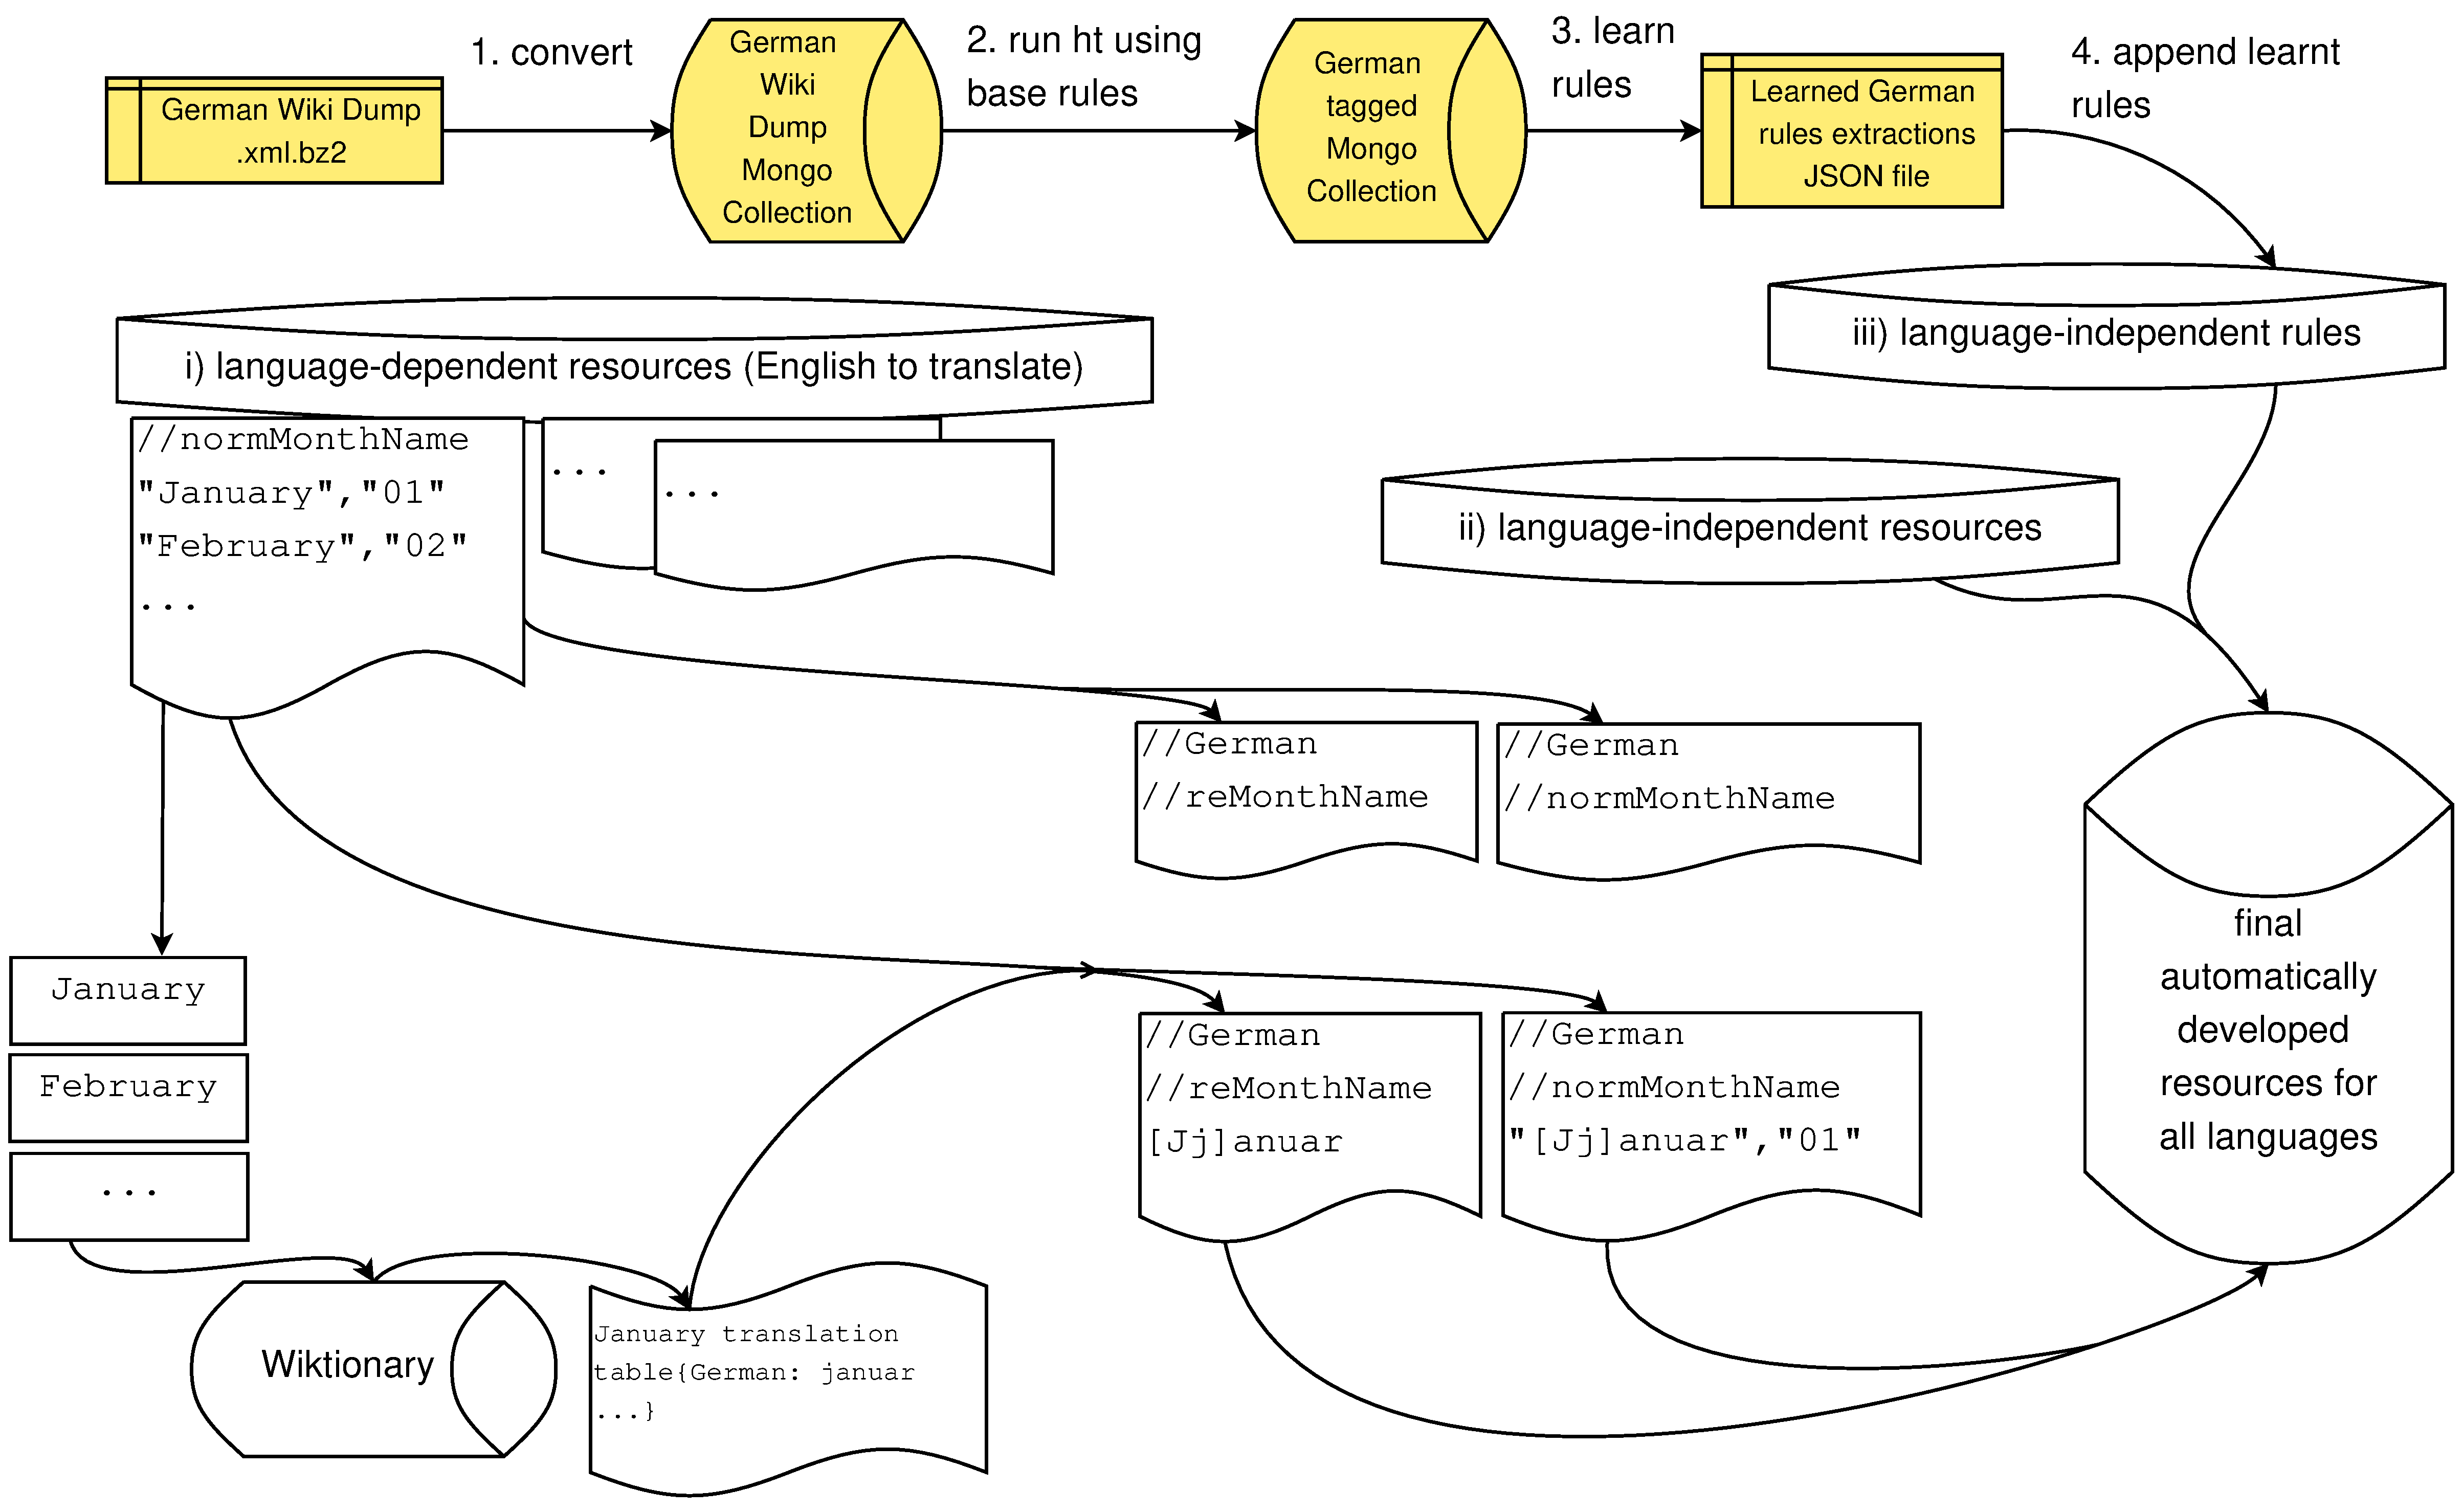
\includegraphics[width=14cm]{Graphics/ht-multilingual-new-3}
	\caption{Overview of Improved Mutlilingual HeidelTime Model - Learning Language-specific Frequent Rules - using Wikipedia.}
	\label{figure:4d}
\end{figure}

\textbf{Learned Rules}\\
In following listing we summarize some of the rules that were learned by our implementation of learning languages specific rules, by analysing respective languages Wikipedia dumps.  \\

\begin{minipage}{\linewidth}
\lstset{caption={Some sample rules learned for different languages.},label={listing:4f}, showspaces=true}
\begin{lstlisting}
// complete date rule for German language
RULENAME="daterules-freq-rule-1",EXTRACTION="%reDayNumber. %reMonthName %reYear4Digit",NORM_VALUE="group(3)-%normMonthName(group(2))-%normDayNumber(group(1))"

// complete date rule for Spanish language
RULENAME="daterules-freq-rule-2",EXTRACTION="%reDayNumber de %reMonthName de %reYear4Digit",NORM_VALUE="group(3)-%normMonthName(group(2))-%normDayNumber(group(1))"

// only year date rule for Finnish language
RULENAME="daterules-freq-rule-3",EXTRACTION="%reYearToken %reYear4Digit",NORM_VALUE="group(2)"

// only year date rule for Finnish language
RULENAME="daterules-freq-rule-4",EXTRACTION="[Vv]uonna %reYear4Digit",NORM_VALUE="group(2)"

// year duration rule for Urdu language 
RULENAME="durationrules-freq-rule-5",EXTRACTION="%reDayNumberWord4Duration %reYearToken",NORM_VALUE="P%normDayNumberWord4Duration(group(1))Y"

// complete date rule for Chinese language
RULENAME="daterules-freq-rule-6",EXTRACTION="%reYear4Digit年%reMonthNumber月%reDayNumber",NORM_VALUE="group(1)-%normMonthNumber(group(2))-%normDayNumber(group(3))"

\end{lstlisting}
\end{minipage}

The first rule, i.e., ``daterules-freq-rule-1" in Listing \ref{listing:4f}, shows the most frequently occurring complete date rule for German language learned by our system. Its extraction part tells that it can extract dates that have reDayNumber followed by dot and space, followed by reMonthName and space, followed by reYear4Digit. For instance, ``20. Januar 2002" can be extracted by this rule. However, there is already a rule (c.f. Listing \ref{listing:4a}) in language independent rules that can extract similar dates.

The second rule, i.e., ``daterules-freq-rule-2" in Listing \ref{listing:4f}, shows the most frequently occurring complete date rule for Spanish language learned by our system. Here the parts of the date are separated by the Spanish word ``de". For instance, ``20 de enero de 2002" can be extracted by this rule. However, such complete dates in Spanish language can already be extracted by one of the rule (c.f. Listing \ref{listing:4a}) in language independent rules. 

The third rule, i.e., ``daterules-freq-rule-3" in Listing \ref{listing:4f}, shows the most frequently occurring only year date rule for Finnish language learned by our system. The rule learnt tells us that in Finnish language year token appears before the year digits. This rule can extract Finnish year only temporal expressions such as the temporal expression ``vuodesta 1971" from the following text\footnote{The Finnish text excerpt is taken from Wikipedia, see \url{https://fi.wikipedia.org/wiki/?curid=30}}.  

\begin{mdframed}[style=MyFrame]
	\raggedright{
		Antti Satuli oli ulkoministeriön palveluksessa \ul{vuodesta 1971} kuolemaansa saakka. Satuli kuoli sairauskohtaukseen ollessaan hiihtomatkalla Lapissa keväällä 2003.
	}
\end{mdframed}

Such a rule that extracts only year temporal expressions is not present in language independent rules; thus, this rule can extract Finnish temporal expressions of year granularity that were not extracted by HeidelTime as of version 2.2.1.

The fourth rule, i.e., ``daterules-freq-rule-4" in Listing \ref{listing:4f}, shows another only year rule learned by our system. This is different from the third rule in that it has the word ``vuonna" itself instead of any pattern name that contains ``vuonna", this is because the word ``vuonna" is not extracted from Wiktionary while making the pattern resources. Such a rule that extract only year temporal expressions is not present in language independent rules; thus, this rule can extract expressions that were not extracted by HeidelTime as of version 2.2.1.

The fifth rule, i.e., ``durationrules-freq-rule-5" in Listing \ref{listing:4f}, shows the a duration rule learned by our system for Urdu language. The rule is reDayNumberWord4Duration followed by space reYearToken. Temporal expressions representing temporal duration in years can be extracted by this rule. For instance, this rule can extract Urdu temporal durations such as \texturdu{پانچ سال}, \texturdu{سات سال}, etc. meaning ``five years" and ``seven years" respectively. However, there is already a similar rule (c.f. rule ``durationrules-freq-rule-1" in Listing \ref{listing:3-lirules}) in language independent rules that can extract such duration temporal expression.

The sixth rule, i.e., ``daterules-freq-rule-6" in Listing \ref{listing:4f}, shows the most frequently occurring complete date rule for Chinese language learned by our system. We can see that reYear4Digit is followed by the Chinese word for year, i.e., 年. Similarly, reMonthNumber is followed by the Chinese word for month, i.e., 月. For instance, this rule can extract Chinese dates such as ``2015年7月29", etc. This rule can extract dates in Chinese that were not extracted using language independent rules as of version 2.2.1 of HeidelTime. 

\textbf{Observations}\\
In general, our system is able to learn simple rules for the different languages (Spanish, German, Finnish, Urdu among others). The simple rules learned are such that some of them are already part of language independent rules. However, we also do learn some rules that are not part of language independent rules. We make following observations about the language specific frequently occurring rules learned by our system. 
\begin{enumerate}[1.]	
	\item Our system was able to learn most frequently occurring order of individual patterns of complete date for various languages such as Spanish, German, Finnish and Chinese.	
	\item Our system was able to learn only year rule for various languages. This rule had two contributing individual patterns, i.e., reYearToken and reYear4Digit, and their correct order along with frequent tokens between them was learned by our system to make the only year rule.
	\item Our system was able to learn only year rule when it had only one contributing individual pattern, i.e., reYear4Digit. The signal word such as `in' was learned and its correct position (before or after) was learned by our system to make this kind of only year rule. For instance, \framebox{\%reYear4Digit \texturdu{میں}} for Urdu language was learned, that translates to \framebox{in \%reYear4Digit} in English. 
\end{enumerate}


%\item 3 iterate over all timexes per document and compare them, based on count - yes 
%-> average number of temporal expressions found per document (old vs new)

%\item 4 iterate over all timexes per document and compare them, based on type - yes
%-> average number of temporal expressions found per type per document (old vs new)

%\item 5 iterate over all timexes per document and compare them, based on normalized value - yes
%-> can draw a graph with normalized years on x-axis and on y axis average number of occurrences in document (old vs new), to find the year that was referred the most

%\item 6 iterate over all timexes per document and compare them, based on abstracted/generalized value (e.g., instead of 2017-11 use YYYY-MM etc.)
%\item 7 iterate over all timexes per document and compare them, based on covered text (i.e., the string which is extracted) -yes

\section{Summary}
In this chapter, we described in detail our contributions to improve the multilingual model of HeidelTime. We started the chapter by discussing the external data sources we use for our work, i.e., Wiktionary, FastText and Wikipedia. In following section, we explained our model, extension of \cite{DBLP:conf/emnlp/StrotgenG15}, that uses Wiktionary to get inflections of patterns while creating the automatically developed resources. Furthermore, we also used FastText, in a separate model, to get inflections. Then, we discussed how we can accommodate unsegmented languages by removing space as delimiter in language independent rules. Finally, we explained our approach to learn frequently occurring temporal patterns as rules. Our system can learn the most frequently occurring order of contributing patterns in the rules and the tokens that separate the patterns.